\section{Event Detection from Group Absenteeism}


Social microblogs such as Twitter and Weibo are experiencing explosive growth, with billions of users globally sharing their daily status updates online.
For example, Twitter has more than 255 million average monthly active users (78\% from mobile) as of March 31, 2014, and an estimated increase of 25\% per year\footnote{http://solomozone.com/tag/revenues/}.
Various studies have shown that Twitter is viable as a social ``sensor'', and holds great promise for detecting and forecasting significant societal events~\cite{bugel2013multilingual,sakaki2010earthquake}.
In recent years, a significant body of research~\cite{aggarwal2012event,hong2012discovering,lappas2009burstiness,lappas2012spatiotemporal,sakaki2010earthquake,sayyadi2009event,watanabe2011jasmine,weng2011event,yin2011geographical} has focused on modeling bursts and increases of user activity in social media.

However, real world events are not only correlated with burst signals, but can also exhibit unusually low levels of activity in social networks.
As shown in Figure 1, a protest in the city of Natal, Brazil began at 5:00 PM (local time) at the Museum of the Republic, with people gradually joining the demonstration. %\footnote{http://www.jb.com.br/pais/noticias/2013/06/17/manifestantes-invadem-cobertura-do-congresso-nacional-em-brasilia/}.
On Twitter, there was an uncharacteristic lull in activity or {\it group absenteeism} behavior from 6:00 PM---8:00 PM on the same day.
%Another example comes from December 24, 2013, southern Brazil experienced widespread flash floods. According to news sources, more than 50,000 people were forced to flee their homes in Minas Gerais and Espirito Santo, in the southern states of Brazil. Immediately following the floods, Twitter activity in this region dropped by 51\%, and reached its lowest point that evening.
%Other examples of \textit{group absenteeism} that we observed from Latin American Twitter activity include bus strikes in Brazil on May 21, 2014, the Iquique earthquake in Chile on April 1, 2014, and a major power supply disruption in Argentina on December 30, 2013.

\begin{figure}[t]
\centering
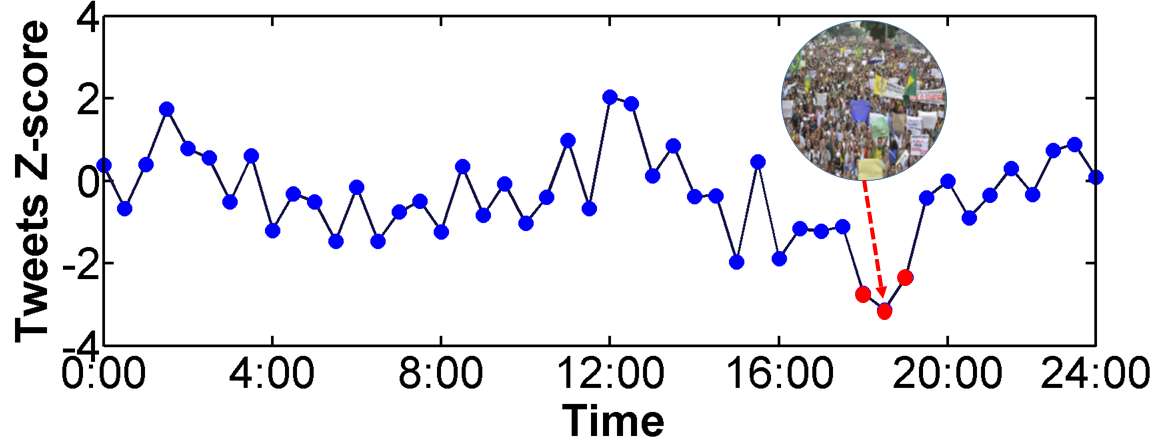
\includegraphics[height=1.1in]{figures/Natal_example1.png}
\caption{Detected group absenteeism in Natal, Brazil beginning at 6:00 PM on June 17, 2013. This absenteeism event coincides with a large protest that happened in the region.}
\vspace{-1em}
\label{fig:natal-protest}
\end{figure}

Investigating this phenomenon of unusually calm behavior online holds enormous potential for understanding localized, disruptive societal events. One recent research work~\cite{chi2015ghost} detects vacant housing areas in China using using Baidu positioning data, which is a practical application of absenteeism study. In this chapter we focus on absenteeism based event detection, and introduce this important topic as a key data mining task for social media analytics.
An \textit{absenteeism} event in social networks can be defined as an event which is characterized by a significant lull in activity such as a sudden, sharp decrease of Twitter volume within a short period of time (and which  often precedes a major burst in re-activity).
This chapter presents the first study to systematically investigate group absenteeism in LBSNs.
Using graph wavelet techniques, we pose this problem as one of group anomaly detection.
%To appropriately incorporate absenteeism concepts into our detection approach, we must first address the following questions:
%\begin{itemize}
%\item What scale should we select to model the absenteeism groups? %Which node should be the central point?
%
%\item What is the most efficient approach to select absenteeism groups that are spatially and temporally localized?
%
%\item How do we model an absenteeism signal for event detection? Even though we have clear examples of real world events which can explain the observed absenteeism, not all absenteeism occurrences can be associated with underlying events. Therefore we must be able to differentiate absenteeism from noisy signals for event detection.
%\end{itemize}

Graph wavelets display two outstanding advantages to study the above
questions: scalability and low computational complexity.
In this scenario, the data objects are embedded in a general graph as vertices.
By employing wavelet transforms on the graph, we can construct a wavelet function with a graph structure, and we are able to select absenteeism groups at different scales.
Lastly, we propose a two-pass group anomaly detection method that first detects absenteeism, and then checks if there is a subsequent burst in activity within a specific time period.
By comparing correlations between the wavelet coefficients of both of these groups, we are able to relate observed absenteeism to a possible real world event.


Our contributions are:
\begin{itemize}
\item We propose the method to modeling group absenteeism as a basis for event detection.
%Even though burst has been extensively discussed in previous work, however, the absenteeism has different patterns and plays an irreplaceable role in event detection.
\item We incorporate graph wavelets as a mechanism to detect the most anomalous subgraphs at different scales. We demonstrate how this is a powerful technique for social media analytics.
\item We propose a novel two-pass event detection method that uses correlation scores between the group depicting \textit{absenteeism} and the group demonstrating increased activity to probabilistically determine the likelihood of an event.
\end{itemize}

%The rest of the chapter is organized as follows. Section~\ref{sec:related} reviews related work and existing methodologies and Section~\ref{sec:preliminaries} formalizes the research problem. In Section~\ref{sec:algorithm}, we first discuss the graph wavelet formalism for group absenteeism detection, and subsequently demonstrate how it can be used for two-pass event detection. Section~\ref{sec:experiment} presents extensive experiments for event detection, and the chapter concludes with a summary of the research in Section~\ref{sec:conclusion}.


\subsection{Problem Statement}
\label{sec:problemformulation}
We focus on the problem of event detection from online social networks, based on the absenteeism behavior observed in user activity in geographically proximal communities or group of cities.
We define this problem as following: \emph{given a graph and \textit{absenteeism score} vector, $\mathbf{G}(V,E,W;f^t)$ at time interval $t$, select a subset $\Sigma \subseteq V$, such that
\vspace{-0.5em}
\begin{eqnarray}
 \label{eq: problem}
    \Sigma=\underset{P\subseteq V, P \mbox{ is compact}}{\arg\min}\ \ \sum_{v_k\in P} {f(k)}
\end{eqnarray} }

A general solution to this problem is using a combinatorial optimization technique, where by defining a constrained objective function over a network one can identify subset of vertices which maximize the corresponding function~\cite{rozenshtein2014event}. Therefore, Equation~\ref{eq: problem} can be modified as:
\vspace{-0.5em}
\begin{eqnarray}
 \label{eq: problem_conventional}
    \Sigma=\underset{P\subseteq V}{\arg\min}\ \ \sum_{v_k\in P} {f(k)}+\lambda \mu(P)
\end{eqnarray}
, where $\mu(P)$ is the compactness penalty function of $P$ (e.g., the sum of distances among
all pairs of the vertices in $P$~\cite{rozenshtein2014event}), and $\lambda$ is the regularization parameter.
Such methods suffer from the following issues:
\begin{enumerate}
\item To define and measure the compactness of subset $P\subseteq V$ is challenging, considering the exponential varieties of complex graphs.
\item To determine a suitable regularization parameter $\lambda$ in the objective function is ambiguous, because simply combining multiple physically different concepts in the objective function makes the optima sensitive to $\lambda$.
\item To solve this objective function is often a \textbf{NP-hard} problem, which makes it unpractical in many real world applications. Sometimes, even the approximate solutions are of high computation complexity, if there are any.
\end{enumerate}

In contrast, our approach proposes a novel, absenteeism based events detection algorithm in social networks using spectral graph wavelet theory.
The graph wavelets focus on the intrinsic geometric structure of the graph by transversing each vertex $v_i\in V$, and mining the topological information of both local and globally centered vertices supports the ability to conduct a multiscale analysis.
In addition, the graph wavelet approach does not introduce any ``subjective'' objective functions or other compactness concepts, and thus provides a fair and low computational method in terms of complexity for identifying abnormal group behavior in a wide variety of application scenarios.

\subsection{Graph Wavelet}
Classic wavelet is called mathematical microscope since it is capable of showing signal abnormality with different scales. In the case of complex networks, graph wavelets render the graph with good localization properties both in frequency and vertex (i.e. spatial) domains. Their scaling property allows us to zoom in/out of the underlying structure of the graph.

It is useful to analyze $f$ by taking into account the intrinsic geometric structure of the graph $\mathbf{G}$. In order to identify and exploit structure of  $f\in \mathbb{R}^N$, the spectral graph $\sigma({\mathcal{L}}):=\{\chi_l\}_{l=0}^{N-1}$ can be used as a dictionary of atoms~\cite{shuman_ACHA_2013}. Thus, $f$ can be decomposed as a linear combination of $\{\chi_l\}_{l=0}^{N-1}$ as
\vspace{-0.5em}
\begin{equation}
\label{eq:graph_fourier}
f(n)= \sum\limits_{l=0}^{N-1}\hat{f}(l)\chi_l(n)
\end{equation}
\vspace{-0.5em}
, where
\vspace{-0.5em}
\begin{equation}
\label{eq:graph_fourier1}
\hat{f}(l):= \sum\limits_{n=0}^{N-1}\chi^*_l(n)f(n)
\end{equation}
$\chi_l$ is called the Fourier frequency of $f(n)$ based on the graph $\mathbf{G}$, and $\hat{f}(l)$ is the corresponding Fourier coefficient.
Equation~\ref{eq:graph_fourier1} and Equation~\ref{eq:graph_fourier} are called Fourier transform and inverse Fourier transform, respectively.
Equation~\ref{eq:graph_fourier1} gives a clear representation of the Fourier components in $f(n)$.
However, information concerning the vertex-location can not be identified from the Fourier transform. To address this issue, Hammond et al.~\cite{hammond2011wavelets} proposed constructing wavelet transforms of functions over the vertices using weighted graphs, described in the following steps:

\begin{enumerate}
\item Define a continuous generating kernel functions $g(x)$ on $\mathbb{R}^+$;
\item Then, select a central vertex $v_a \in {V}$ and scale $s$, set the frequency coefficients as $g(s\lambda_l)\chi^*_l(a)$ for each frequency component $\chi_l$;
\item Finally, sum up all those frequency components $\chi_l$.
\end{enumerate}
In this way, the graph wavelet at central vertex $v_a$ is constructed as:
\vspace{-0.5em}
\begin{equation}
\label{eq:graphwaveletdefinition}
\psi_{s,a}(n) = \sum\limits_{l=0}^{N-1}g(s\lambda_l)\chi_l^*(a)\chi_l(n)
\end{equation}
After setting up the graph wavelet, the wavelet coefficients for $f$ can be defined as
\vspace{-0.5em}
\begin{equation}
\label{eq:graph_graphwavelet}
W_f(s,a)=<\psi_{s,a}, f>=\sum\limits_{l=0}^{N-1}g(s\lambda_l)\hat{f}(a)\chi_l(n)
\end{equation}



\subsection{Two-pass Event Detection Model}

We intend to propose a two-pass absenteeism based event detection algorithm. The underlying rationale of this algorithm is based on the following concepts.
\begin{enumerate}
\item As discussed above, distribution of $f$ can be well reconstructed by the $J$ scaling and $NJ$ wavelet coefficients. Each of those normalized wavelet coefficients $W'_f(s,a)$ represents a distribution pattern of $f$ on $\mathbf{G}$.
It is equivalent to saying that $\psi_{s,a}$ represents a special distribution pattern, which shares a large and uniform value around the central vertex with scale $s$.
\item When a significant event occurs, preceded by group absenteeism behavior in social networks, such as a severe earthquake or a massive protest, it is likely to be succeeded by a spike or burst in online user activity.
With this observation, we can represent an absenteeism behavioral pattern as $\psi_{s_l,a_l}$ at time $l$ centering at vertex $v_{a_l}$, and a burst related pattern as $\psi_{s_{\tau,a_\tau}}$ at time $\tau$ centering at vertex $v_{a_\tau}$. We assume the burst pattern happens within the time window size of $L$ after absenteeism pattern is identified. Further, a notion of response time can represented using the time difference $t_{rsp}=\tau-l$.
\item Both absenteeism and burst signal must show a strong correlation, especially if they occur in close proximity spatially and temporally.
For instance, taking the power-cut-off for instance, usually only people who live in the affected area will ``yield at " this event a lot because it brings inconvenience to their life. However, people who live outside of the affected areas would hardly mention this event. Thus, to measure the correlation between absenteeism pattern and burst pattern is proposed as:
\begin{equation}
\label{eq:eventsimilarity}
\rho(\psi_{s_l,a_1}, \psi_{s_\tau,a_\tau})= \frac{<\psi_{s_l,a_1}, \psi_{s_\tau,a_\tau}>}{||\psi_{s_l,a_1}||\cdot ||\psi_{s_\tau,a_\tau}||}
\end{equation}
Based on these concepts, the higher the correlation, the higher probability that burst patterns is caused by the preceding group absenteeism. When $\rho$ is above the threshold (threshold is set at 0.5), we infer that an event occurred and that it evolved on social networks into distinct phases: first group absenteeism, followed by a spike or burst in user activity.
\end{enumerate}


\subsection{Experiments}
We seek to answer the following questions using our model:
To appropriately evaluate our detection approach, we seek to answer the following questions:
\begin{itemize}
\item What scale should we select to model the absenteeism groups? %Which node should be the central point?
\item What is the most efficient approach to select absenteeism groups that are spatially and temporally localized?
\item How do we model an absenteeism signal for event detection? Even though we have clear examples of real world events which can explain the observed absenteeism, not all absenteeism occurrences can be associated with underlying events. Therefore we must be able to differentiate absenteeism from noisy signals for event detection.
\item Given a time period, what is the recall and precision to identify events using group absenteeism as signals?
\end{itemize}
\subsection{Datesets}
We will uses tweets from 22 countries in Latin America that were collected over 24 months, from May 2013 to May 2015.
